%%%%%%%%%%%%%%%%%%%%%%%%%%%%%%%%%%%%%%%%%%%%%%%%%%%%%%
%%%%%%%%%            TikZ Example            %%%%%%%%%
%%%%%%%%%%%%%%%%%%%%%%%%%%%%%%%%%%%%%%%%%%%%%%%%%%%%%%
\documentclass[11pt]{article}

%################################################
%########            Packages            ########
%################################################

\usepackage{tikz}    % Diagrams
\usetikzlibrary{positioning,arrows,shadows,shapes,patterns,decorations.pathmorphing}    % Some TikZ libraries

%>>>>>>>>>>>>>>>>>>>>>>>>>>>>>>>>>>>>>>>>>
%>>>>>>            Setup            >>>>>>
%>>>>>>>>>>>>>>>>>>>>>>>>>>>>>>>>>>>>>>>>>

\tikzset{
modal/.style={
    >=stealth',
    shorten >=1pt,
    shorten <=1pt,
    auto,
    node distance=2cm,
    semithick
},
state/.style={
    circle,
    draw,
    minimum size=0.5cm,
    fill=gray!15
},
point/.style={
    circle,
    draw,
    inner sep=0.5mm,
    fill=black
},
sees/.style={
    ->
},
seen/.style={
    <-
},
seens/.style={
    <->
},
rfl/.style={
    ->,
    in=120,
    out=60,
    loop,
    looseness=5
}}

\newcommand{\stack}[1]{{\def\arraystretch{0.6}\begin{array}{c} #1 \end{array}}}

%::::::::::::::::::::::::::::::::::::::::::::::::
%::::::            Front Matter            ::::::
%::::::::::::::::::::::::::::::::::::::::::::::::

\begin{document}

\textbf{Example 1:}

\begin{center}
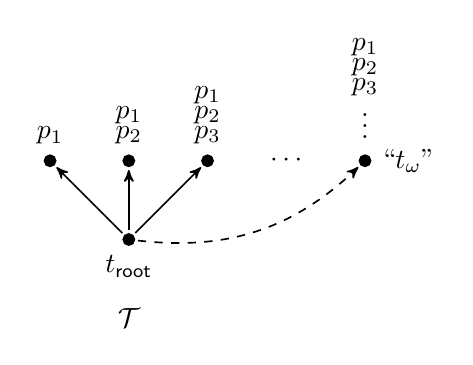
\begin{tikzpicture}[modal, node distance=1cm]
\node[point]    (p1)    [label=above:$p_1$]    {};
\node[point]    (p2)    [right of=p1, label=above:$\stack{p_1 \\ p_2}$]    {};
\node[point]    (p3)    [right of=p2, label=above:$\stack{p_1 \\ p_2 \\ p_3}$]    {};
\node[point]    (r)     [below of=p2, label=below:$t_\mathsf{root}$]    {};
\node           (con)   [right of=p3]    {$\cdots$};
\node[point]    (pw)    [right of=con, label=above:$\stack{p_1 \\ p_2 \\ p_3 \\ \vdots}$, label=right:``$t_\omega$'']    {};
\node           (T')     [below of=r]    {$\mathcal{T}$};

\path    (r)    edge[sees]    (p1);
\path    (r)    edge[sees]    (p2);
\path    (r)    edge[sees]    (p3);
\path    (r)    edge[sees,dashed, bend right=25]    (pw);
\end{tikzpicture}
\end{center}

\textbf{Example 2:}

\begin{center}
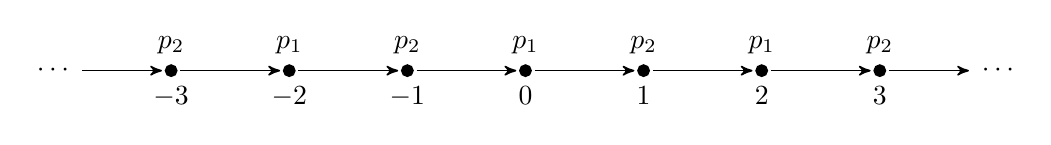
\begin{tikzpicture}[modal, node distance=1.5cm]
\node[point]    (0)    [label=above:$p_1$, label=below:$0$]    {};
\node[point]    (1)    [right of=0, label=above:$p_2$, label=below:$1$]    {};
\node[point]    (2)    [right of=1, label=above:$p_1$, label=below:$2$]    {};
\node[point]    (3)    [right of=2, label=above:$p_2$, label=below:$3$]    {};
\node           (r)    [right of=3]    {$\cdots$};
\node[point]    (-1)   [left of=0, label=above:$p_2$, label=below:$-1$]    {};
\node[point]    (-2)   [left of=-1, label=above:$p_1$, label=below:$-2$]   {};
\node[point]    (-3)   [left of=-2, label=above:$p_2$, label=below:$-3$]   {};
\node           (l)    [left of=-3]    {$\cdots$};

\path    (l)    edge[sees]    (-3);
\path    (-3)   edge[sees]    (-2);
\path    (-2)   edge[sees]    (-1);
\path    (-1)   edge[sees]    (0);
\path    (0)    edge[sees]    (1);
\path    (1)    edge[sees]    (2);
\path    (2)    edge[sees]    (3);
\path    (3)    edge[sees]    (r);
\end{tikzpicture}
\end{center}

\textbf{Example 3:}

\begin{center}
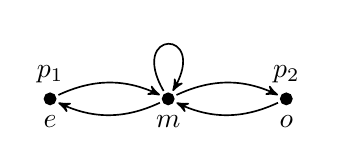
\begin{tikzpicture}[modal, node distance=1.5cm]
\node[point]    (e)    [label=above:$p_1$, label=below:$e$]    {};
\node[point]    (m)    [right of=e, label=below:$m$]    {};
\node[point]    (o)    [right of=m, label=above:$p_2$, label=below:$o$]    {};

\path    (e)    edge[sees, bend left=25]    (m);
\path    (m)    edge[sees, bend left=25]    (e);
\path    (o)    edge[sees, bend left=25]    (m);
\path    (m)    edge[sees, bend left=25]    (o);
\path    (m)    edge[rfl, in=60, out=120, looseness=30]    (m);
\end{tikzpicture}
\end{center}

\textbf{Example 4:}

\begin{center}
\begin{tikzpicture}[modal]
\node    (r)                         {$t_\mathsf{root}$};
\node    (1p1)  [above left=5mm of r]    {$p_1$};
\node    (1p2)  [above left=5mm of 1p1]  {$p_2$};
\node    (1p3)  [above left=5mm of 1p2]  {$p_3$};
\node    (1pd)  [above left=-2mm of 1p3]  {\rotatebox[origin=c]{-10}{$\ddots$}};

\node    (2p1)  [above=5mm of r]         {$p_1$};
\node    (2p2)  [above=5mm of 2p1]       {$p_1$};
\node    (2p3)  [above=5mm of 2p2]       {$p_2$};
\node    (2p4)  [above=5mm of 2p3]       {$p_3$};
\node    (2pd)  [above=1mm of 2p4]       {$\vdots$};

\node    (3p1)  [above right=5mm of r]   {$p_1$};
\node    (3p2)  [above right=5mm of 3p1] {$p_1$};
\node    (3p3)  [above right=5mm of 3p2] {$p_1$};
\node    (3p4)  [above right=5mm of 3p3] {$p_2$};
\node    (3p5)  [above right=5mm of 3p4] {$p_3$};
\node    (3pd)  [above right=-2mm of 3p5] {\rotatebox[origin=c]{80}{$\ddots$}};

\node    (con)  [below right=1mm of 3p3]  {$\ddots$};
\node    (cont) [below right=1mm of con]  {$\vdots$};

\node    (wp1)  [right=5mm of r]          {$p_1$};
\node    (wp2)  [right=5mm of wp1]        {$p_1$};
\node    (wp3)  [right=5mm of wp2]        {$p_1$};
\node    (wp4)  [right=5mm of wp3]        {$p_1$};
\node    (wpd)  [right=0mm of wp4]        {$\dots$};


\path    (r)    edge[sees]    (1p1);
\path    (r)    edge[sees]    (2p1);
\path    (r)    edge[sees]    (3p1);
\path    (r)    edge[sees]    (wp1);

\path    (1p1)  edge[sees]    (1p2);
\path    (1p2)  edge[sees]    (1p3);

\path    (2p1)  edge[sees]    (2p2);
\path    (2p2)  edge[sees]    (2p3);
\path    (2p3)  edge[sees]    (2p4);

\path    (3p1)  edge[sees]    (3p2);
\path    (3p2)  edge[sees]    (3p3);
\path    (3p3)  edge[sees]    (3p4);
\path    (3p4)  edge[sees]    (3p5);

\path    (wp1)  edge[sees]    (wp2);
\path    (wp2)  edge[sees]    (wp3);
\path    (wp3)  edge[sees]    (wp4);
\end{tikzpicture}
\end{center}

\pagebreak
\textbf{Example 5:}

\begin{center}
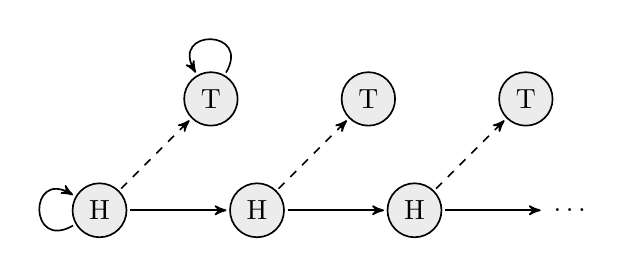
\begin{tikzpicture}[modal]
\node[state]    (h1)                       {H};
\node[state]    (h2)    [right of = h1]    {H};
\node[state]    (h3)    [right of = h2]    {H};
\node[state]    (t1)    [above right of = h1]    {T};
\node[state]    (t2)    [above right of = h2]    {T};
\node[state]    (t3)    [above right of = h3]    {T};
\node           (e)     [right of = h3]    {\dots};

\path    (h1)    edge[rfl, in=150, out=210]    (h1);
\path    (t1)    edge[rfl]    (t1);

\path    (h1)    edge[sees]    (h2);
\path    (h2)    edge[sees]    (h3);
\path    (h3)    edge[sees]    (e);

\path    (h1)    edge[sees,dashed]    (t1);
\path    (h2)    edge[sees,dashed]    (t2);
\path    (h3)    edge[sees,dashed]    (t3);
\end{tikzpicture}
\end{center}

\textbf{Example 6:}

\begin{center}
\begin{tikzpicture}[node distance=1ex]
\node    (A->B)                                {$A \rightarrow B$};
\node    (A&-B)    [below=of A->B]             {$A \wedge \neg B$};
\node    (-A)      [below left=7mm of A&-B]    {$\neg A$};
\node    (A)       [below=of -A]               {$A$};
\node    (x-A)     [below=of A]                {$\times$};
\node    (B)       [below right=7mm of A&-B]   {$B$};
\node    (A2)      at (x-A -| B) [yshift=-7mm] {$A$};
\node    (-B)      [below=of A2]               {$\neg B$};
\node    (x-B)     [below=of -B]               {$\times$};

\path    (A&-B)    edge[-]    (-A);
\path    (A&-B)    edge[-]    (B);
\path    (B)       edge[-]    (A2);

\node    (1)    [left=2cm of A->B]    {1.};
\node    (2)    at (1 |- A&-B)        {2.};
\node    (3)    at (1 |- -A)          {3.};
\node    (4)    at (1 |- A)           {4.};
\node    (5)    at (1 |- A2)          {5.};
\node    (6)    at (1 |- -B)          {6.};

\path    (5)    edge[-,dashed]    (A2);
\path    (6)    edge[-,dotted]    (-B);

\node    (r1)   [right=2cm of A->B]   {P};
\node    (r2)   at (r1 |- A&-B)       {P};
\node    (r3)   at (r1 |- -A)         {($\rightarrow$), 1};
\node    (r4)   at (r1 |- A)          {($\wedge$), 2};
\node    (r5)   at (r1 |- A2)         {($\wedge$), 2};
\node    (r6)   at (r1 |- -B)         {($\wedge$), 2};
\end{tikzpicture}
\end{center}


\end{document}